\documentclass[a4paper,dutch,fleqn]{exam}

\usepackage[english]{babel}

\usepackage{babel} % voor nederlandse afbreekregels e.d.
\usepackage{hyperref} % voor links, hier niet gebruikt
\usepackage{graphicx} % voor importeren van figures, hier niet gebruikt
\usepackage{tabularx} % voor tabellen met controle over kolombreedte, hier niet gebruikt
\usepackage{booktabs} % voor nettere tabellen dan de standaard
\usepackage{enumerate} % voor controle over nummering van items
\usepackage{amssymb,amsmath,amsthm,amsfonts} % van de AMS, voor nettere math
\usepackage{qtree} % voor het maken van mooie bomen, hier niet gebruikt
\usepackage{mathabx} %voor het \notdivides commando, niet gebruikt
\usepackage{adjustbox}
\usepackage{listings}
\usepackage{color}
\usepackage{pifont}
\usepackage{comment}
\usepackage{pdfpages}
\usepackage{tikz}
\usetikzlibrary{automata,arrows}
\usepackage{algorithm} % pseudocode
\usepackage[noend]{algpseudocode} %pseudocode 
\usepackage{sectsty}
\usepackage{amsbsy}
\usepackage[utf8]{inputenc}
\usepackage[english]{babel}
\usepackage{wrapfig}
\usepackage{csquotes}
\usepackage{biblatex}
\bibliography{bibliography}

\renewcommand\thesubsection{\thesection \alph{subsection}}
\newcommand{\s}{\text{*}}

%\DeclareGraphicsExtensions{.pdf,.png,.jpg}


%\renewcommand{\baselinestretch}{0.9} 

%\sectionfont{\fontsize{12}{15}\selectfont}

\renewcommand{\qedsymbol}{\hfill \emph{QED}}

% document variables:
\title{uSquam - Project Idea Document}
\newcommand{\coursename}{uSquam, a mobile crowdsourcing platform}
\newcommand{\doctitle}{Project Idea Document}
\newcommand{\deadline}{March 11, 2017}
\newcommand{\examdate}{\deadline}
\newcommand{\authors}{Group 3}

%\newcommand{\cmark}{\ding{51}}%
%\newcommand{\xmark}{\ding{55}}%

\newcommand{\itab}[1]{\hspace{0em}\rlap{#1}}
\newcommand{\tab}[1]{\hspace{.2\textwidth}\rlap{#1}}


% http://tex.stackexchange.com/questions/80113/hide-section-numbers-but-keep-numbering

% http://tex.stackexchange.com/questions/110328/formatting-a-logical-pd-derivation:
\newcommand{\fgh}[1]{\fvline%
  \makebox[0pt][l]{{%
      \raisebox{-1.4ex}[0pt][0pt]{\rule{#1}{\arrayrulewidth}}}}%
  \hspace*{\fitchindent}}
  
  \lstset{language=Java,
%alles tussen "//(*" en "*)" wordt als TeX code verwerkt
	escapeinside={//(*}{*)}} 
 


\newcommand*\xor{\mathbin{\oplus}}
% Fill these in:

% if you use algorithms, this is a nice one:
% http://www.lirmm.fr/~fiorio/AlgorithmSty/
%\usepackage[algo2e]{algorithm2e}

\makeatletter

% http://detexify.kirelabs.org/classify.html

% Use Sans-Serif font:
\renewcommand{\familydefault}{\sfdefault}


\coverextraheadheight[1cm]{0cm}
\coverfirstpageheader{TECHNISCHE UNIVERSITEIT DELFT\\
Faculteit Elektrotechniek, Wiskunde en Informatica\\ \vspace{.5cm}}{}{\includegraphics[clip]{logo}}

\setlength{\parskip}{\medskipamount}
\setlength{\parindent}{0pt}

\makeatother

%%%%%%%%%%%%%%%%%%%%%%%%%%%%%%%%%%%%%%%%%%%%%%%%%%%%%%%%%%%%%%%%%%%%%%%%%%%%%%%%
%% document start
%%%%%%%%%%%%%%%%%%%%%%%%%%%%%%%%%%%%%%%%%%%%%%%%%%%%%%%%%%%%%%%%%%%%%%%%%%%%%%%%
\begin{document}

\thispagestyle{empty}

\begin{center}


\includegraphics[scale=0.3]{image03}
%\vspace*{2cm}
%{\huge \coursename}
\begin{center}
    \line(1,0){450}
\end{center}

\vspace{2cm}
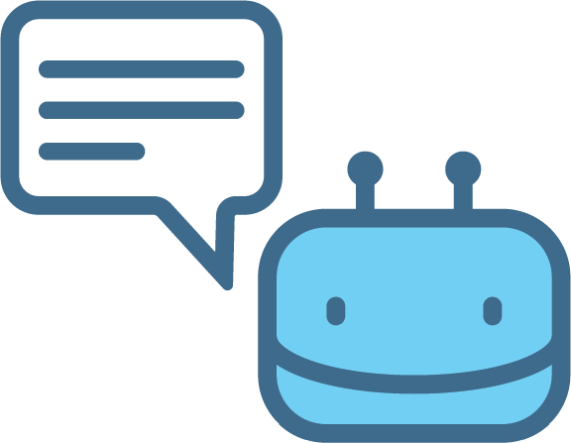
\includegraphics[scale=0.45]{chatbot}
\vspace{2cm}
{ \Large \\ \doctitle \\ Information Retrieval (IN4325) \\}
\vspace{0.5cm}
{\Large \textbf{deadline:} \examdate \\ \vspace{1cm} Group 3}

\end{center}

\newpage

\section{Introduction}
Think about all the time that you have wasted on commuting, standing in line, waiting for your food or simply being bored. Now imagine that there was a solution to convert that time into fun and an easy way to earn some money simultaneously. The solution that you are wondering about is our chatbot called \emph{uSquam}. It is a worker-side human computation platform which allows people to perform crowdtasks through a chat service. Current crowdwork is carried out in traditional desktop-oriented interfaces, such as CrowdFlower or Mechanical Turk. By offering microtasks in a mobile environment, human computation tasks can be made more accessible and more attractive to a larger audience. It can be beneficial for those with busy schedules and it solves the problem of having to deal with various user interfaces.

\textbf{Objectives and customers} \\
The goal of our project is to design and develop uSquam: a general purpose crowdsourcing platform which allows people to perform crowdtasks in the form of a conversation with a chatbot. uSquam means \emph{'anywhere'} in Latin, representing the flexibility and easiness of use of the platform. The platform will be generic enough to support various tasks and applications. The chatbot will have its own pool of tasks, as well as an API to push more tasks to the pool. This means that our project involves two types of customers:

\begin{itemize}
\itemsep0em 
\item The requesters, who publish tasks via the requesters API and gather the answers from workers.
\item The workers, who perform tasks via the chatbot for a small reward.
\end{itemize}

This so-called requesters API allows the management and creation of tasks, such that some content is shown/given to a worker (e.g. text, an image, a map location etc), then various questions are asked about this content. To answer such questions the worker can click buttons, type text, upload images, audio files, videos. The tasks content can be gathered from public data sources (e.g. Twitter, Instagram), local data sources (e.g. Dropbox) or it can be generated by workers (e.g. 'take a picture at Starbucks in Amsterdam').

uSquam will handle the distribution of tasks across workers and will  gather, store and validate the results from workers. It will also take care of the reward system. The final product would optimally have a web interface on the requester's side where they can simply add and edit new tasks. The platform will be created in such a way that it can easily be extended to different Messenger services. However, due to the scope of the project, we will restrict ourselves to only implement one messenger front-end and we decided to use Telegram. 

\textbf{Implementation of task pipelines}\\
In order to demonstrate our platform's functionality, we will create three task pipelines to implement three task use cases. The three task types will be as follows: 
\begin{enumerate}
\itemsep0em 
\item Based on data gathered from a global data source, like Twitter or Flickr, and use uSquam to process the data.
\item Based on a local data source, like a set of images stored on Dropbox, and use uSquam to process the data.
\item Use uSquam for situational content generation, for example the chatbot could ask the worker to make picture at a certain place and time.
\end{enumerate}

\textbf{Structure of the document}\\
In this document we will analyze and explain our idea in more detail. In the first chapter we will discuss the relevance of the project to this course. Next, we will look into the benefits uSquam offers and the challenges that we expect to face. Chapter 4 gives an overview of the platform's requirements that are prioritized using the MoSCoW-method. This will be used as an reference during the development phase of the project. Chapter 5 explains the internal design of the system with a flow diagram of the major system components and mockups of the chatbot interface. Chapter 6 describes the methods and metrics by which the success of our project and product can be evaluated. Chapter 7 and 8 will present our execution plan and business plan, respectively. These plans illustrate how uSquam's fullest potential can be achieved by taking potential business and scheduling risks into account.

\newpage

\section{Course relevance}
Our product is going to apply at least four Information Retrieval concepts that are relevant to the course. Namely, web crawling, human computation, quality control and natural language processing.

\textbf{Web crawling} \\
The task pipelines need to contain a part that is responsible for data acquisition on the requestors side. This data needs to be gathered from public data sources such as Twitter (content with a given hashtag) and Instagram. The input data stream should be retrieved and filtered using a web crawler and an ElasticSearch instance. The gathered media content will be used as task content for the workers. Web crawling is critical in Information Retrieval as it is primarily used for retrieving documents from the Internet, saving them to a collection and making these documents ready to be indexed by an IR system. It provides a method for the 'retrieval' part of a data processing pipeline.

\textbf{Human computation} \\
The main goal of our project is to develop a worker-side human computation platform which allows people to perform crowdtasks in a mobile environment. Each of the available tasks listed by our chatbot will have a set of questions to be answered by the worker. The answering of those questions is essentially the human computation part of the project. In order to ensure the validity of the answers provided by our users, we are going to introduce quality control measures. For example, the worker's answer could be validated by  asking gold standard questions \cite{oleson2011programmatic}. These are questions of which we know the answer and they enable us to check the correctness of the answer provided by the worker. This way we can gain confidence about the user's trustworthiness and honesty in performing human computation. Based on this, the worker could be warned or even blocked after providing several wrong answers.  

As we are going to implement a human computation platform, we also need to deal with areas related to human interaction. How do people interact with a chatbot? How can we make the chatbot more likeable and human-like? How can we motivate the workers to perform tasks? How can the chatbot support workers to perform tasks faster? We will need to keep this kind of considerations into account while designing the platform.

\textbf{Natural language processing} \\
The chatbot is to be used by workers. Tasks to be performed should be retrieved according to free-text queries of users and also by means of conversations between the worker and the bot. In such a conversation the chatbot could ask for contextual information (e.g. current location or mood) or the bot could question the response of the worker. “Thank you for sending me the picture I requested. Are there any bikes in your picture?”

In order to enable the chatbot to use more tree-based conversations rather than linear communication, we will need to perform natural language processing. This will especially be challenging when handling the first interaction with the worker since the worker could either ask for a new task, a list of all available tasks, his current balance or something unexpected. The worker will express his queries using natural language and our platform needs to be able to understand the worker's intent. 
Natural language processing plays an important role in Information Retrieval as it the process that searches for meaning in text and can be used for satisfying an information need. 

\section{Innovation and challenges}

The usage of a chat environment introduces opportunities and constraints that are not present in current crowdsourcing platforms. Compared to a service like Amazon Mechanical Turk or CrowdFlower, a chatbot is more convenient since it does not require the installation of a new application and it is available anywhere from any device. There is however no way to have a customized user interface; we are limited by what the chat application offers. As a result, it will be harder to perform user authentication and to validate input from workers. Below we will discuss the innovation opportunities of our chatbot and the challenges that go along with it. The prototype that we will create mostly has technical challenges, while the finished product will have others as well.

\subsection{State of the art}
Current crowdsourcing platforms are offered in conventional desktop-oriented user interfaces, such as Amazon Mechanical Turk and CrowdFlower. Since these platforms are less accessible, they lack the situational aspect of tasks. By offering crowdtasks in a mobile environment, information can be collected in the physical world without space and time boundaries. For example, the chatbot could ask a worker to make a selfie at Starbucks between 1PM and 3PM today. 
In addition, the accessibility of mobile environments enable requesters to gain a wide and flexible workforce audience \cite{gupta2012mclerk}. Since people are less motivated to perform crowdtaks when they have a laptop with them, they will be more motivated to do this while commuting to their work or while waiting in line for a store. Besides, the results collected from the chatbot could be more clear as a conversational UI will gather answers that are better structured (one question at a time) and it could even give feedback on the worker's responses. 

At last, uSquam will be a generic platform, meaning that it will be able to support various tasks. It will be general enough so that later if a requester decides to implement a new task or a new task type, they don't need to touch the code of the platform. They will only have to implement a new pipeline for the task type. The requesters will also be able to generate their task content based on various data sources, which could be public and local. 

\subsection{Prototype challenges}
\textbf{Flexible architecture}
At the core of the system lies its architecture. Since the platform needs to be generic, the architecture should be designed in a flexible manner in order to allow requesters to build various tasks. This is mentioned as a challenge because it requires a well-designed architecture of the whole system. We will need to consider architectural trade-offs between system quality attributes, such as flexibility versus performance, flexibility versus reliability and performance versus security. In order to deal with this challenge, we will use the architecture trade-off analysis method (ATAM) for risk mitigation in consultation with Pavel \cite{kazman1998architecture}. Our initial design can be found in section \ref{architecture}.

\textbf{Quality control}
Quality control will be a vital component of the whole system. If false answers are accepted, it degrades the quality of the data collected from workers. As a consequence, the reputation of our service could be lowered. Therefore, we will need to apply some quality control, which will not be possible for every type of task. Simple types of answers, such as “yes” or “no” and numbers, could be validated using techniques such as \emph{gold standard questions} or \emph{agreement schemes} \cite{oleson2011programmatic}. However, with image processing and object recognition this task is already harder to do. Besides this, some sort of cheat detection should also be incorporated in the chatbot to avoid abuse.

\textbf{Tree-based communication}
The chatbot will need to have interactive conversational skills, meaning that it should be able to deal with conversation scripting and state handling. Until now there has not been a lot of projects that apply this in a crowdsourcing context. The ones that do, such as CleverBot, still resemble the idea of a linear conversation though. We are going to try to improve this and make workers feel like they are interacting with a human-like chatbot. 

Since this is a very complex concept and we have to keep in mind that our project has a limited time frame, we will implement a simplified model. The logic of the chatbot will mainly be constructed as a tree or as something that is similar to a state machine. Intents and conversation states will be mapped to a branch of code that will react in a way based on the current state \cite{states}. Whenever slots are encountered, those get stored into a conversation state. As the user types a response, the process repeats. In the future this could be extended by using a machine learning model that can be trained on a series of messages and be trained to predict the next message. This way the system starts using older conversational content to make more accurate predictions on what messages to send.

\textbf{User experience}
An additional challenge is that current natural language processing (NLP) and machine learning technologies are not refined enough to offer excellent user experiences. User errors and confusion can increase during worker's the first interaction with the chatbot when the bot needs to express its functionality to new workers and set the correct expectations. Therefore, we will need to implement some kind of error handling in case the chatbot does not understand the worker's response. Requesters should also be made aware of this problem and know how to define clear tasks, thereby decreasing the chance of confusion. Related to this challenge is the downfall of many generic platforms: most platforms only work well horizontally and do not perform well on specific use cases. We will need to make sure that various tasks can easily be created by changing the task pipelines and connecting it with different data sources. 

\textbf{Reward system}
Another challenge is related to the reward system. While the general idea of transferring money seems simple, it needs to be very secure and working flawlessly. For the prototype, we might use a fake virtual currency for simplicity's sake.

\subsection{Product challenges}
\textbf{Discovery of users}
The application would not be functional without an active user base. A major challenge will be finding requesters and many suitable workers that can perform the available tasks. Telegram has created a bot that tells users about other bots. However, this would not be sufficient for us to reach a large audience. Workers could be discovered with a targeted marketing campaign to promote uSquam. This campaign should clarify the concept of crowdwork and the benefits of performing microtasks in a chat service. Requesters and investors could be found by advertising, networking and referrals.

\textbf{Maintenance difficulties}
The goal of making our product as generic as possible might cause trouble in later stages of the project. Not all chat services offer the same features and not all data sources can produce the data format that can be imported in our application. 

\section{Requirements specification}
In this section the requirements of the chatbot will be specified and prioritized using the MoSCoW method \cite{highsmith2001agile}. This is a prioritization technique used in software development to determine the importance the stakeholders place on the fulfillment of each requirement. The term MoSCoW itself is an acronym derived from the first letter of each of four prioritization types (Must have, Should have, Could have, and Would like but won't get). The crowdsourcing platform that we are going to build needs to fulfill the following requirements: \\

\textbf{Must have requirements}
\begin{itemize}
\itemsep0em 
\item As a requester I would like to view a list of existing tasks through the use of an API.
\item As a requester I would like to add new tasks through the use of an API.
\item As a requester I would like to attach media content to the tasks that I create.
\item As a requester I would like the chatbot to allow answers of type text and type list.
\item As a requester I would like to edit existing tasks through the use of an API.
\item As a requester I would like to get the answers given by workers through the use of an API.
\item As a worker I would like the chatbot to be passive so that I will not be disturbed when I am busy with other activities. 
\item As a worker I would like to be able to perform the tasks in the Telegram UI.
\item As a worker I would like to to request a new task from the platform.
\item As a worker I would like to get rewarded with money by the chatbot for the tasks that I have performed.
\end{itemize}
 
\textbf{Should have requirements} 
\begin{itemize} 
\itemsep0em 
\item As a requester I would like the chatbot to use 10\% “gold” standard data to validate the workers answers.
\item As a requester I would like the chatbot to warn workers that have given an unexpected answer according to the implemented quality control technique(s).
\item As a requester I would like to add a new task type (new pipeline) through the use of an API.
\item As a worker I would like to be able to get a list of all available tasks with corresponding title, reward and expected execution time.
\item As a worker I would like to be able to select the task that I want to perform.
\item As a worker I would like to be informed if I have completed a task successfully.
\item As a worker I would like to get the current total amount of money that I have earned by performing tasks. 
\end{itemize} 

\textbf{Could have requirements} 
\begin{itemize}
\itemsep0em 
\item As a requester I would like to view, add and edit tasks through a web interface.
\item As a requester I would like to add a new task type (new pipeline) through a web interface.
\item As a requester I would like to get an overview of all tasks that have been fulfilled. 
\item As a requester I would like the chatbot to be able to use tree-based conversations in order to get more elaborate and context-aware answers. The bot should at least be able to ask one extra question based on the worker's response to the initial task.
\item As a requester I would like to add tasks that are based on the GPS location of the worker so that I can get data with a situational aspect.
\item As a requester I would like the chatbot to block workers that have given more than three unexpected answers (according to the implemented quality control techniques).
\item As a worker I would like the chatbot to recommend me a task based on the amount of (spare) time I have to perform the task.
\item As a worker I would like to receive feedback on the answers that I give to questions.
\item As a worker I would like like to be able to perform the tasks in chat services other than Telegram (e.g. Messenger).
\item As a worker, I would like to be able to request the chatbot a list of newly added tasks.
\end{itemize} 

\textbf{Won't have requirements} 
\begin{itemize}
\itemsep0em 
\item As a requester I would like to add new tasks through the chatbot. 
\item As a requester I would like to get suggestions about the content of my tasks based on the data already entered.
\item As a customer I would like the chatbot to sanity check the entered data.
\end{itemize}

\subsection{Use cases}
  In order to demonstrate our chatbot's functionality, we will create several data pipelines to implement three specific task use cases. These use cases will be based on data collection for sentiment analysis and will be as following:
\begin{enumerate}
\itemsep0em 
\item \underline{Global content scraped from Twitter} \\
The chatbot shows the worker a tweet and asks about the sentiment of the message: is it expressed positively, negatively or neutral? The worker can either pick one of the three options or indicate that he or she is not sure. Sometimes tweets are about negative subjects but are expressed positively and vice versa, which can be confusing. 
\item \underline{Local content provided by the requester} \\
The chatbot shows the worker an image of a group of people and asks him to describe the ambience in the picture. The worker can respond with a freely expressed text.
\item \underline{Content retrieval} \\
The chatbot asks the worker to take a selfie with a defined face expression, e.g. the worker could be asked to take a selfie while looking angry.
\end{enumerate}

\section{Flow diagram}
\label{architecture}
We have previously mentioned what our platform will need to be able to accomplish and how we are going to bring it to the market. In this section we are going to explain how we imagine our software to work internally. An example task will be used as a demonstration to make the analysis easier to follow.

Let's imagine a research group that is building a face-recognition system that can identify emotions in the faces you feed to it. In order to implement such a system, the team requires annotated data, so pictures of faces for which they know which expression the face shows. Our application would offer multiple ways to obtain this kind of data: either the team sends their own database of images for the workers to tag, or get images from social networks like Twitter with a hashtag \#selfie or we could ask the user to send us selfies with a given expression. Let's assume our research team prefers the third use case concerning content retrieval the best. We will now go through the whole process of creating a new task on our platform to the final answers in ElasticSearch. 

\subsection{Create a new task} 
Our software needs to provide an API for the requester side which allows requesters to create new task pipelines, define the answer types and rewards. As shown in our should-have requirements, it seems to be the easiest if we provide a website where requesters can create such tasks with a graphical user interface. 

\begin{figure}[!ht]
    \centering
    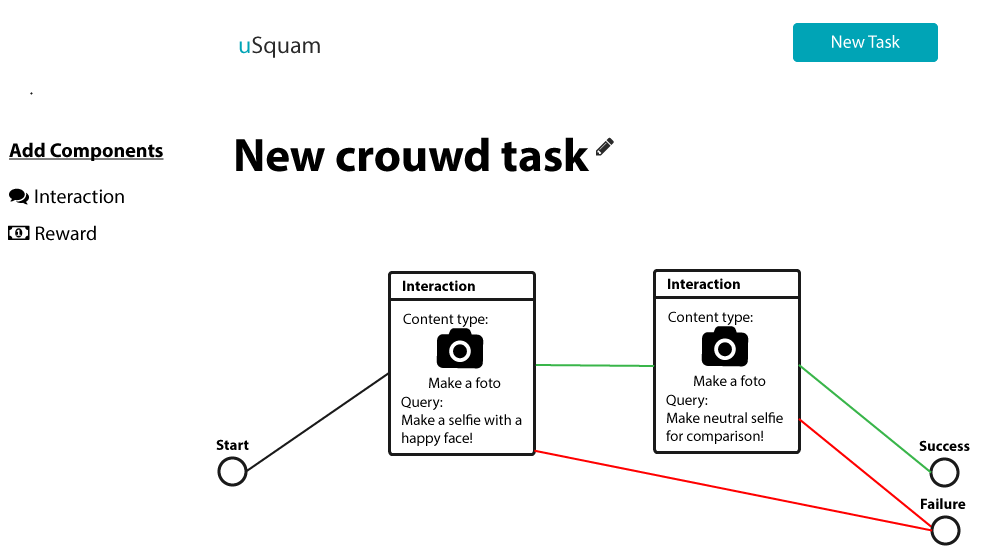
\includegraphics[scale=0.5]{image02}
    \caption{Potential Web UI for requesters API}
\end{figure}

Figure 1 shows how such a website could look like. Basically, the requester needs to construct a flow from Start to Success with interaction elements that define what the worker needs to do. In this case we define two interactions, first the worker should create a photo with a happy face and if that succeeded (the green connection) the worker should also create a neutral reference photo so the researcher team can train their system to find the difference. However, something could go wrong, like the worker does not want to give the chat app permissions to his camera or the user types a response instead of making a photo. In that case the interaction leads to the fail status. Once the requester is happy with their task, they can submit it. Then the website will convert the diagram to a JSON object which is sent to the server to store it and register it in the TaskManagement system.

The TaskManager will keep track of all the existing tasks and register them in the system. That could mean sorting the tasks by requester or by category. The TaskManager should be able to return the list of available tasks, or give a task which matches a value of meta-data. This describes the requester side, so let's approach the system's core components from the other side, that of the workers.

\begin{figure}[!ht]
    \centering
    \includegraphics[scale=0.45]{image00}
    \caption{Flow diagram of uSquam}
\end{figure}

\subsection{Executing a task}
One of the main features that our platform will provide is the chatbot interface for workers which will be available on a Messaging platform. As with all crowdsourcing examples, the workers decides when he or she has time to perform tasks. Therefore, our chatbot will be passive. So a usual case would be a worker sitting on the train or waiting for his pizza to come out of the oven, wanting to use their downtime usefully. The worker would tell the chatbot that he is willing to perform a task and the chatbot will immediately offer a task for the worker to do. 

In our architecture we view the chatbot's interaction with the worker as a separate task which could be performed by any chatbot service, it's just receiving text or media, and sending other messages in return. Therefore we decided to split this from our worker's API and make the latter universal, such that it might be extended to work with any Messaging application that employs a Chatbot API. For testing purposes we will however create a chatbot interface for the Telegram messenger. 

Any chatbot interface will interact with the InteractionManager (IM), our actual workers API, which handles the state of the interaction, decides which query or media to send next. The IM receives a state and a message from the chatbot. If no state was received like for the first interaction, the IM uses the default state which handles workers requests like a new task, the users balance or an overview of all tasks. 

Once the user has started a task, the InteractionManager loads that Task and returns the task ID, the state ID and the query of the state. Next, the user will respond to the chatbot which forwards the response, together with the state ID and task ID. Now the InteractionManager gets the task and state object, and determines what to do given the response of the user. For every response the IM sends an updated TaskAnswer to the TaskManager that stores the answers in the database (and/or on ElasticSearch).

This interaction continues until the user breaks the interaction by leaving the conversation or reaching the end of the task. Once the interaction finishes, the IM sends an empty state ID and task ID, such that the next request from the chatbot is handled by the idle state again. 

\begin{wrapfigure}{l}{0.35\textwidth}
 \begin{center}
    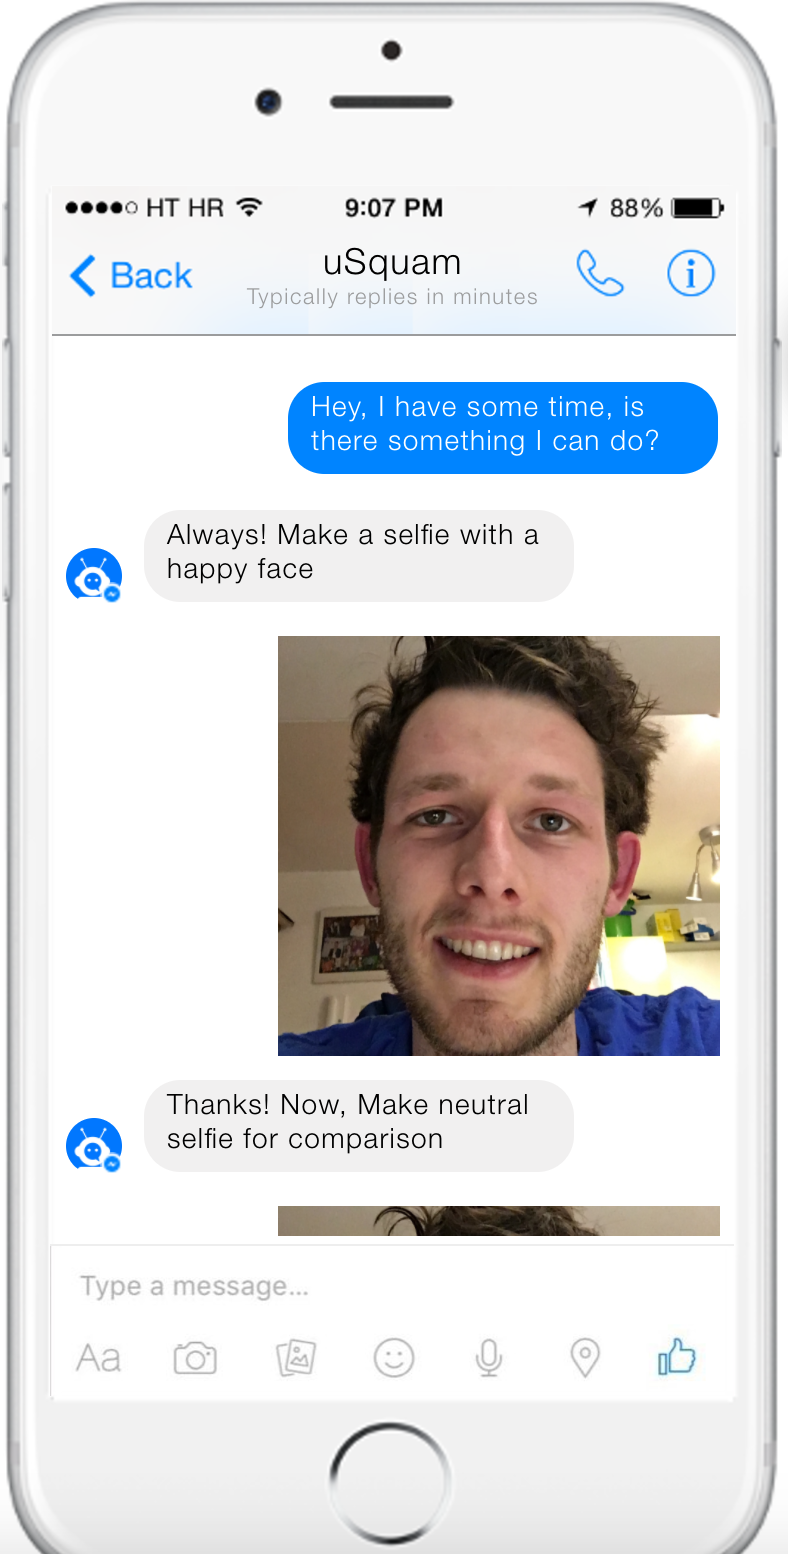
\includegraphics[width=0.3\textwidth]{image01}
  \end{center}
    \caption{A mockup of the chatbot}
\end{wrapfigure}

\subsection{Conclusion \& outlook}
In this document, we have explained our current understanding of the project and how we aim to successfully create an application which fulfills the requirements that we have composed with our product owner Pavel. 
To summarize, our platform's backend will consist of three components: 
\begin{enumerate}
\item The requesters API, a simple RESTful API to create, update and delete task pipelines. 
\item The TaskManager, which handles the storage of incoming tasks, the set of available tasks, and which task to provide next to the InteractionManager.
\item The InteractionManager, which - given a current task - handles the interaction with the chatbot, which can be any chatbot application based only on the task and the input. So the InteractionManager could be a pure function without external effects. 
\end{enumerate}

Obviously, due to the project's limited timeframe, this view is a simplified consideration of the system. In the future we might want to add more advanced features to improve the chatbot's performance. The InteractionManager might be extended with advanced Natural Language Processing functionality in order to give the worker more freedom in responding or to make the chatbot more human-like. Especially the first interaction with the chatbot might be hard if we would like to implement requests such as: "show me my current balance". 
We also need to handle authentication of both sides. The requesters side can be handled with an authentication token, but for the workers side we would need to implement authentication techniques in the chatbot or in the messenger application's user management. We will need to keep these considerations into account during the construction phase of the final application.

\newpage 

\section{Evaluation \& Success metrics}
To get a clear picture of where our project is heading to, it is important to plan stepwise evaluation strategies such as key evaluation questions, types of evaluation measures and experimental design \cite{patton2002two}. These evaluation strategies are crucial for our key resources including customers – requesters and workers, stakeholders and the development team.
In this case, we will make a separation between the evaluation of project success and product success. 
 
\subsection{Project success}
The success factors of a project are the elements or activities required for ensuring the success criteria of the project. Key evaluation questions would include:
\begin{itemize}
\itemsep0em 
\item Have all must-have and should-have requirements specifications been successfully implemented?
\item Has the project been finished within the specified time frame and budget? 
\item Have the resources, that are made available for the project, been optimally used by the project team?
\item Has each team member participated actively in the project and made a valuable contribution to the project outcome?
\end{itemize}

\subsection{Product success}
The success factors of a product are the elements or features that make sure that the product works as intended. Key evaluation questions about the product quality would include:
\begin{itemize}
\itemsep0em 
\item Does the platform meet the user needs of both types of customers - the requesters and the workers?
\item Is the application achieving its objective of providing an easy-to-use worker-side human computation platform which allows people to perform crowdtasks in a mobile environment?
\item Does our product have a WOW factor? 
\item How appropriate are the processes compared with quality standards?
\end{itemize}

These key questions on product success could be answered by performing a customer satisfaction survey. The following type of questions could be proposed to workers: 
\begin{itemize}
\itemsep0em 
\item Would you like to use the uSquam chatbot?
\item Would you dedicate at least 10 minutes of your time regularly to perform microtasks using uSquam?
\item Did you experience any confusion during your conversation with the chatbot?
\item Was the expected execution time of the task consistent with your completion time?
\item Was it clear to you which tasks you could perform and how you could perform them?
\item Did you find the proposed reward motivating? If no, what kind of reward would you find motivating?
\end{itemize}

The following type of questions could be proposed to requesters: 
\begin{itemize}
\itemsep0em 
\item Would you like to use the uSquam platform?
\item Were you able to add/ edit the tasks you wanted to the chatbot's taskpool?
\item Was it clear to you how the requesters API works?
\item Did you find the collected results satisfying? If not, what could have been improved?
\end{itemize}

\subsection{Evaluation measures}
Evaluation measures or success metrics must be implemented with focus on accuracy, efficiency, appropriateness and quality control which can be achieved using measures like precision and recall for the local information retrieval process. In the case of uSquam, we could measure the fraction of tasks that have been completed successfully by workers and the fraction of answers that was validated as correct.

Evaluation measures with respect to:
\begin{itemize}
\itemsep0em 
\item Marketing include – Monthly Unique visits, Customer Acquisition Cost (CAC) and Organic traffic vs Paid traffic.
\item Stakeholders include - Total monthly/annual recurring revenue, annual contract value and Lifetime value.
\item Customer success include – Net promoters score (NPS) which evaluates Customer experience management, Customer support and Customer feedback.
\end{itemize}
 
Experimental design must ensure that the following criteria are met - Consistency and standards, Aesthetic and minimalist design, Help and documentation, User control and freedom, Flexibility and efficiency of use \cite{heuristics}.

\section{Execution plan}
We have decided to execute the project in five phases that are based on the Unified Process (UP) approach \cite{jacobson1999unified}. This approach is an iterative and incremental software development process framework. Every phase has its initial focus but during every phase other work will also be done to reduce task switching. 

\begin{itemize}
\itemsep0em 
\item \textbf{Phase 1: Inception (February 17 until March 3)} \\
This is the official start for the project and during this phase we have created a team, chosen a project and designed our first draft of the system architecture. The activities in this phase mainly existed of team meetings and meetings with Pavel. These activities were executed with the whole team together and concluded with a pitch.

\item \textbf{Phase 2: Elaboration (March 3 until March 10)} \\
This phase requires the team to formalise and motivate the project topic. This phase results in  our first deliverable, the project idea document. For this document we held two extensive team meetings to discuss the chatbot's requirements and to sketch the application's flow diagram. Remi and Dimitris focused on the challenges and relevance of the project, Anshul and Elvan focused on the prioritization of the requirements and the business plan, and Jan addressed the final sketch of the flow diagram. 

\item \textbf{Phase 3: Construction (March 10 until April 7)} \\
During this phase the prototype will be built using the Scrum methodology. The construction phase will last four sprints in total. In the next paragraph an overview will be given of the goals of each sprint and the responsibilities assigned to each member.

\item \textbf{Phase 4: Transition (April 7 until  April 13)} \\
Transition is the last phase of the project. During this phase the application will be tested, demonstrated and delivered to the teacher. This phase also includes our final presentation.
\end{itemize}

\subsection{Construction phase} 
This phase will be executed in four one-week sprints which will start each Friday at midnight beginning on Friday, March 10th. Each week we will hold two team meetings, namely on Tuesday and Thursday. Each Thursday we will also meet with Pavel to discuss our progress and to make sure that the final application meets his user needs.  

Each sprint will be concluded with an intermediate deliverable, meaning that it will not officially be delivered to the teacher but it will be used to keep the team on schedule. This way we will be able to tackle issues early and discuss them with Pavel.

The sprints will be organized as follows:

\begin{itemize}
\item \textbf{Sprint 1 (March 10  - March 17)} \\
\textbf{Deliverable:} A basic set-up of the MongoDB database, requesters API and workers API \\

\textbf{Task division} \\
\underline{Jan:} Initialize and configure the MongoDB database, set-up basic requesters API (add/ send basic task using JSON file) \\
\underline{Remi:} Initialize and configure local data source \\
\underline{Anshul:} Research how ElasticSearch works \\
\underline{Elvan:} Research how the Telegram API works, set-up basic workers API (get tasks command) \\
\underline{Dimitris:} Explore the Twitter API, set-up twitter crawler in Python

\item \textbf{Sprint 2 (March 17 -  March 24)} \\
\textbf{Deliverable:} A fully working requesters API and chatbot, initial implementation of the three task pipelines \\

\textbf{Task division} \\
\underline{Jan \& Dimitris:} Implementation requesters API (extension task content, edit tasks command, get results command) \\
\underline{Remi \& Anshul:} Implementation task manager, generate test calls to requesters API \\
\underline{Elvan:} Implementation workers API (perform tasks, store answers in MongoDB), set-up state handling for conversational chatbot

\item \textbf{Sprint 3 (March 24 - March 31)} \\
\textbf{Deliverable:} Full implementation of the pipelines, workers response validation, set-up reward system \\
\textbf{Task division} \\
\underline{Jan \& Dimitris:} Implementation and testing of the three use cases \\
\underline{Remi \& Anshul:} Application quality control technique (gold standard question) \\
\underline{Elvan:} Set-up reward system and link it with MongoDb, add getResults command for workers API \\

\item \textbf{Sprint 4 (March 31 - April 7)} \\
\textbf{Deliverable:} Implementation of task recommendation and task choice, set-up web UI for requesters API \\
\textbf{Task division} \\
\underline{Jan \& Dimitris:} Improvements of the chatbot's state handling, execution of additional integration tests \\
\underline{Remi:} Set-up web UI for requesters API \\
\underline{Elvan \& Anshul:} Implementation of task recommendation/ task choice based on available time of worker.
\end{itemize}

\section{Business plan}
Our business plan can be found as a separate attachment on the following page \cite{osterwalder2010business}.

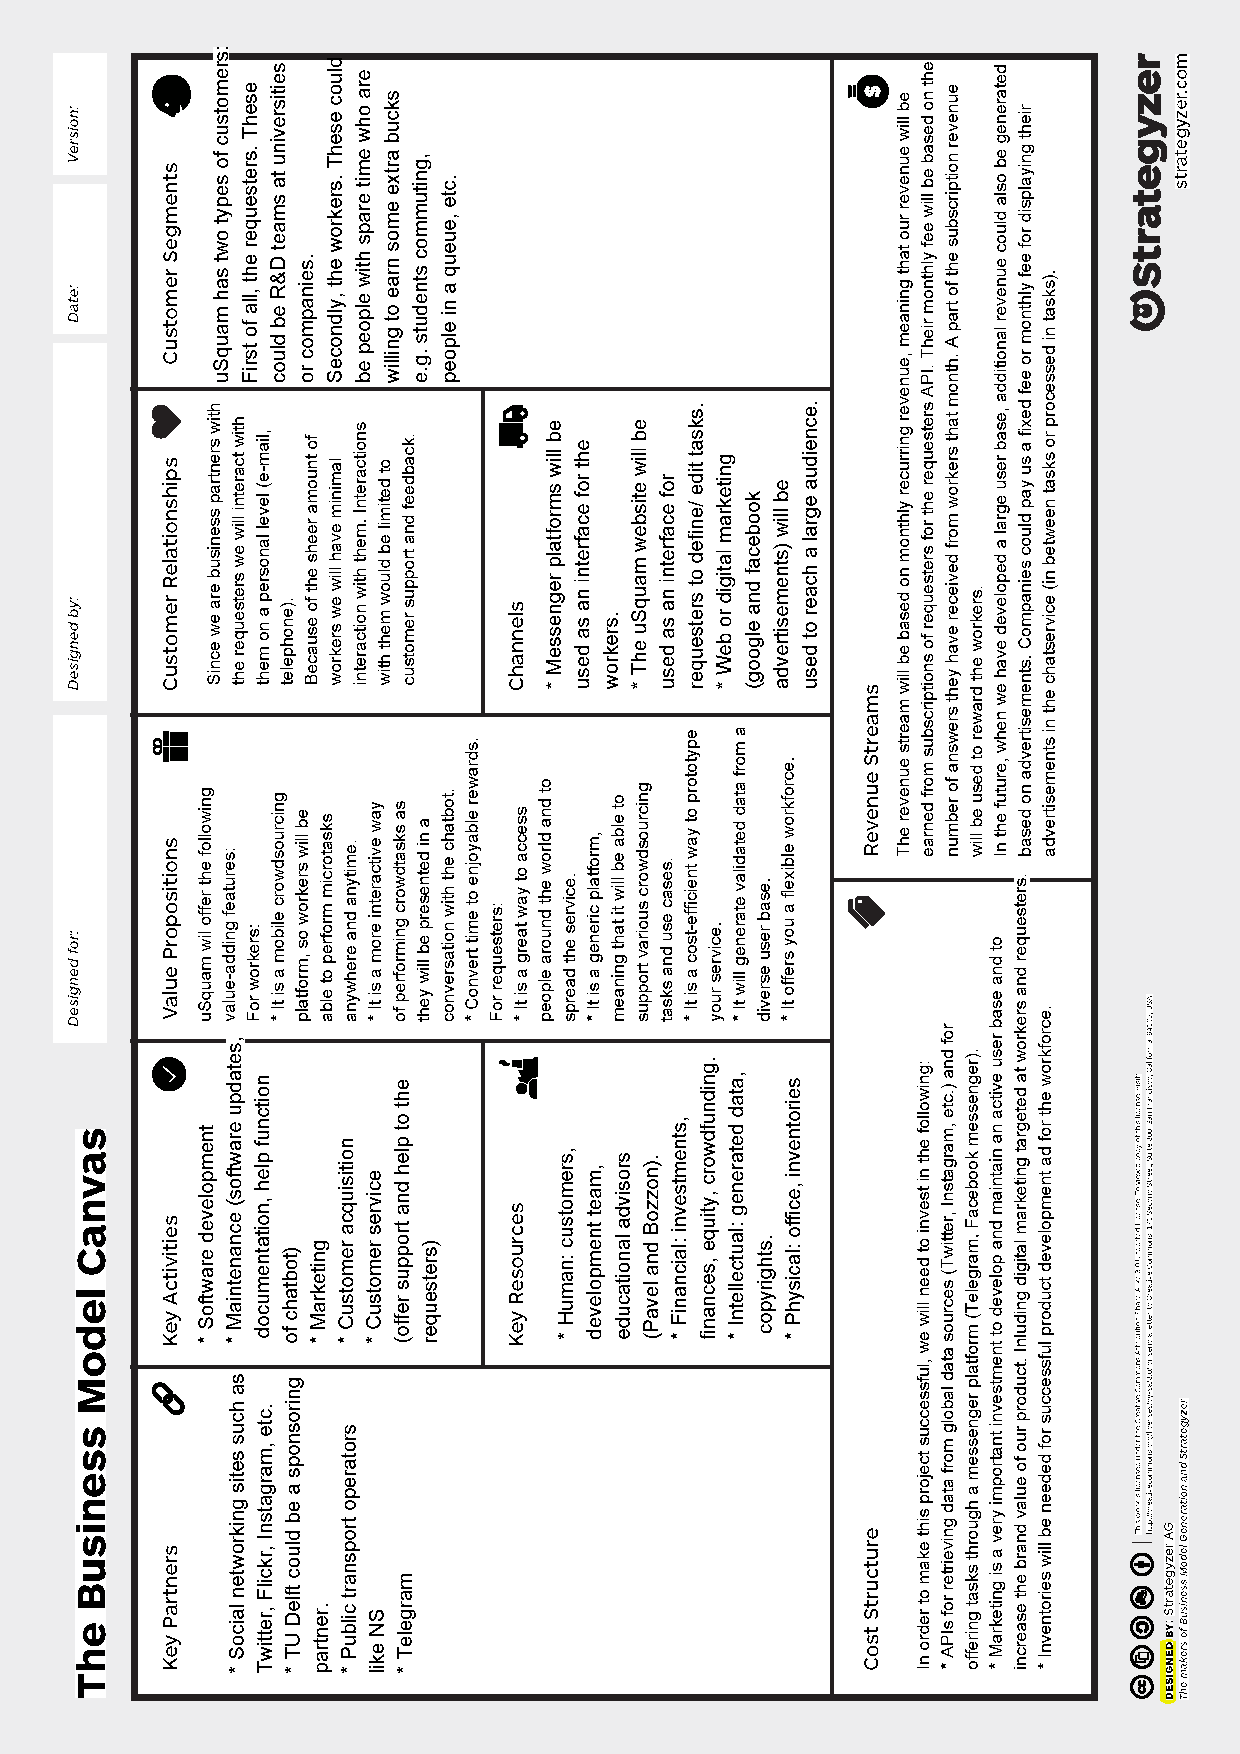
\includepdf[pages={1}]{the-business-model-canvas.pdf}

\newpage 

\printbibliography


\end{document}
%%%%%%%%%%%%%%%%%%%%%%%%%%%%%%%%%%%%%%%%%%%%%%%%%%%%%%%%%%%%%%%%%%%%%%%%%%%%%%%%
